%package list
\documentclass{article}
\usepackage[top=3cm, bottom=3cm, outer=3cm, inner=3cm]{geometry}
\usepackage{multicol}
\usepackage{graphicx}
\usepackage{url}
%\usepackage{cite}
\usepackage{hyperref}
\usepackage{array}
%\usepackage{multicol}
\newcolumntype{x}[1]{>{\centering\arraybackslash\hspace{0pt}}p{#1}}
\usepackage{natbib}
\usepackage{pdfpages}
\usepackage{pgffor}
\usepackage{multirow}
\usepackage[normalem]{ulem}
\useunder{\uline}{\ul}{}
\usepackage{svg}
\usepackage{xcolor}
\usepackage{listings}
\usepackage{tikz}
\lstdefinestyle{ascii-tree}{
    literate={├}{|}1 {─}{--}1 {└}{+}1 
  }
\lstset{basicstyle=\ttfamily,
  showstringspaces=false,
  commentstyle=\color{red},
  keywordstyle=\color{blue}
}
%\usepackage{booktabs}
\usepackage{caption}
\usepackage{subcaption}
\usepackage{float}
\usepackage{array}

\newcolumntype{M}[1]{>{\centering\arraybackslash}m{#1}}
\newcolumntype{N}{@{}m{0pt}@{}}


%%%%%%%%%%%%%%%%%%%%%%%%%%%%%%%%%%%%%%%%%%%%%%%%%%%%%%%%%%%%%%%%%%%%%%%%%%%%
%%%%%%%%%%%%%%%%%%%%%%%%%%%%%%%%%%%%%%%%%%%%%%%%%%%%%%%%%%%%%%%%%%%%%%%%%%%%
\newcommand{\itemEmail}{@unsa.edu.pe}
\newcommand{\itemStudent}{Andre Hilacondo Begazo
Gonzalo Layme Mamani
Andre Delgado Allpan
Sebastian Chirinos Negron
Gabriel Soto Ccoya}
\newcommand{\itemCourse}{Programación Web 2}
\newcommand{\itemCourseCode}{20231001}
\newcommand{\itemSemester}{III}
\newcommand{\itemUniversity}{Universidad Nacional de San Agustín de Arequipa}
\newcommand{\itemFaculty}{Facultad de Ingeniería de Producción y Servicios}
\newcommand{\itemDepartment}{Departamento Académico de Ingeniería de Sistemas e Informática}
\newcommand{\itemSchool}{Escuela Profesional de Ingeniería de Sistemas}
\newcommand{\itemAcademic}{2023 - A}
\newcommand{\itemInput}{Del 05 Junio 2023}
\newcommand{\itemOutput}{Al 12 Junio 2023}
\newcommand{\itemPracticeNumber}{05}
\newcommand{\itemTheme}{Django}
%%%%%%%%%%%%%%%%%%%%%%%%%%%%%%%%%%%%%%%%%%%%%%%%%%%%%%%%%%%%%%%%%%%%%%%%%%%%
%%%%%%%%%%%%%%%%%%%%%%%%%%%%%%%%%%%%%%%%%%%%%%%%%%%%%%%%%%%%%%%%%%%%%%%%%%%%

\usepackage[english,spanish]{babel}
\usepackage[utf8]{inputenc}
\AtBeginDocument{\selectlanguage{spanish}}
\renewcommand{\figurename}{Figura}
\renewcommand{\refname}{Referencias}
\renewcommand{\tablename}{Tabla} %esto no funciona cuando se usa babel
\AtBeginDocument{%
	\renewcommand\tablename{Tabla}
}

\usepackage{fancyhdr}
\pagestyle{fancy}
\fancyhf{}
\setlength{\headheight}{30pt}
\renewcommand{\headrulewidth}{1pt}
\renewcommand{\footrulewidth}{1pt}
\fancyhead[L]{\raisebox{-0.2\height}{
\includegraphics[width=3cm]{img/logo_episunsa.png}}}
\fancyhead[C]{\fontsize{7}{7}\selectfont	\itemUniversity \\ \itemFaculty \\ \itemDepartment \\ \itemSchool \\ \textbf{\itemCourse}}
\fancyhead[R]{\raisebox{-0.2\height}{
\includegraphics[width=1.2cm]{img/logo_abet}}}
\fancyfoot[L]{Job Board}
\fancyfoot[C]{\itemCourse}
\fancyfoot[R]{Página \thepage}

% para el codigo fuente
\usepackage{listings}
\usepackage{color, colortbl}
\definecolor{dkgreen}{rgb}{0,0.6,0}
\definecolor{gray}{rgb}{0.5,0.5,0.5}
\definecolor{mauve}{rgb}{0.58,0,0.82}
\definecolor{codebackground}{rgb}{0.95, 0.95, 0.92}
\definecolor{tablebackground}{rgb}{0.8, 0, 0}

\lstset{frame=tb,
	language=bash,
	aboveskip=3mm,
	belowskip=3mm,
	showstringspaces=false,
	columns=flexible,
	basicstyle={\small\ttfamily},
	numbers=none,
	numberstyle=\tiny\color{gray},
	keywordstyle=\color{blue},
	commentstyle=\color{dkgreen},
	stringstyle=\color{mauve},
	breaklines=true,
	breakatwhitespace=true,
	tabsize=3,
	backgroundcolor= \color{codebackground},
}

\begin{document}
	
	\vspace*{10px}
	
	\begin{center}	
		\fontsize{17}{17} \textbf{ Informe de Laboratorio \itemPracticeNumber}
	\end{center}
	\centerline{\textbf{\Large Tema: \itemTheme}}
	%\vspace*{0.5cm}	

	\begin{flushright}
		\begin{tabular}{|M{2.5cm}|N|}
			\hline 
			\rowcolor{tablebackground}
			\color{white} \textbf{Nota}  \\
			\hline 
			     \\[30pt]
			\hline 			
		\end{tabular}
	\end{flushright}	

	\begin{table}[H]
		\begin{tabular}{|x{4.7cm}|x{4.8cm}|x{4.8cm}|}
			\hline 
			\rowcolor{tablebackground}
			\color{white} \textbf{Estudiante} & \color{white}\textbf{Escuela}  & \color{white}\textbf{Asignatura}   \\
			\hline 
			{\itemStudent \par \itemEmail} & \itemSchool & {\itemCourse \par Semestre: \itemSemester \par Código: \itemCourseCode}     \\
			\hline 			
		\end{tabular}
	\end{table}		
	
	\begin{table}[H]
		\begin{tabular}{|x{4.7cm}|x{4.8cm}|x{4.8cm}|}
			\hline 
			\rowcolor{tablebackground}
			\color{white}\textbf{Laboratorio} & \color{white}\textbf{Tema}  & \color{white}\textbf{Duración}   \\
			\hline 
			\itemPracticeNumber & \itemTheme & 04 horas   \\
			\hline 
		\end{tabular}
	\end{table}
	
	\begin{table}[H]
		\begin{tabular}{|x{4.7cm}|x{4.8cm}|x{4.8cm}|}
			\hline 
			\rowcolor{tablebackground}
			\color{white}\textbf{Semestre académico} & \color{white}\textbf{Fecha de inicio}  & \color{white}\textbf{Fecha de entrega}   \\
			\hline 
			\itemAcademic & \itemInput &  \itemOutput  \\
			\hline 
		\end{tabular}
	\end{table}
	
	\section{Tarea}
	\begin{itemize}
		\item Elabore un primer informe grupal de la aplicacion que desarrollara durante este semestre.
        \item Utilicen todas las recomendaciones dadas en la aplicación library.
        \begin{enumerate}
        \item Los grupos pueden estar conformado por 1 a 4 integrantes.
        \item Solo se presenta un informe grupal.
        \item Solo se revisa un repositorio. (El unico que este en el informe grupal).
        \item Todos los integrantes del grupo tienen una copia del laboratorio e informe en su repositorio privado.
        \item Todos los integrantes deben pertenecer al mismo grupo de laboratorio.
        \item El docente preguntara en cualquier momento a un integrante sobre el proyecto, codigo fuente, avance.
        \end{enumerate}
	\end{itemize}
 
\newpage
	\section{Equipos, materiales y temas utilizados}
	\begin{itemize}
		\item Sistema Operativo (GNU/Linux de preferencia).
		\item VIM 9.0.
		\item Git 2.39.2.
		\item Cuenta en GitHub con el correo institucional.
		\item Python.
		\item Entorno virtual.
        \item Django.
	\end{itemize}
 
	\section{URL de Repositorio Github}
	\begin{itemize}
		\item \textcolor{red}{URL del Repositorio GitHub principal}.
		\item \href{https://github.com/GonzaloRail/Laoboratorio_05_PWEB.git}{\color{blue}\texttt{https://github.com/GonzaloRail/Laboratorio05.git}}
		\item \textcolor{brown}{URL de los repositorios individuales}.
        \begin{enumerate}
        \item \textbf{ANDRE HILACONDO BEGAZO}
        \begin{itemize}
            \item \href{https://github.com/ahilacondo/pweb2-laboratorios/tree/main/lab05}{\color{blue}\texttt{https://github.com/ahilacondo/pweb2-laboratorios}}
        \end{itemize}
        \item \textbf{GONZALO LAYME MAMANI}
         \begin{itemize}
            \item \href{https://github.com/GonzaloRail/myParteLab05PWEB}{\color{blue}\texttt{https://github.com/GonzaloRail/myParteLab05PWEB}}
        \end{itemize}
        \item \textbf{ANDRE DELGADO ALLPAN}
        \begin{itemize}
            \item \href{https://github.com/andre98652/my-first-blog}{\color{blue}\texttt{https://github.com/andre98652/my-first-blog}}
        \end{itemize}
        \item \textbf{SEBASTIAN CHIRINOS NEGRON}
        \begin{itemize}
            \item \href{https://github.com/BastleyNait/Blog-en-Django}{\color{blue}\texttt{https://github.com/BastleyNait/Blog-en-Django}}
        \end{itemize}
        \item \textbf{GABRIEL SOTO CCOYA}
        \begin{itemize}
            \item \href{https://github.com/GabSoto/JOB-s}{\color{blue}\texttt{https://github.com/GabSoto/JOB-s}}
        \end{itemize}
        \end{enumerate}
	\end{itemize}
 
	\section{Resolución del Ejercicio}
	\subsection{Explicación del proyecto}
    \begin{itemize}	
    \item Nos concentramos en realizar una plataforma en línea \textcolor{red}{donde los empleadores pueden publicar ofertas de trabajo y los candidatos pueden buscar y postular a dichas ofertas.}
    
    \begin{minipage}{0.6\textwidth}
        \item Características generales:
        \begin{enumerate}
            \item \textbf{Registro de usuarios:} Los empleadores y los candidatos se registran en plataforma utilizando un nombre de usuario y una contraseña.
            \item \textbf{Autenticación de usuarios:} Los usuarios pueden iniciar sesión y cerrar sesión en la plataforma.
            \item \textbf{Publicación de ofertas de trabajo:} Los empleadores pueden crear y publicar nuevas ofertas de trabajo especificando un título, una descripción, los requisitos y la ubicación.
            \item \textbf{Búsqueda de ofertas de trabajo:} Los candidatos pueden buscar ofertas de trabajo por título, ubicación o categoría.
            \item \textbf{Detalles de las ofertas de trabajo:} Los candidatos pueden ver los detalles de una oferta de trabajo, incluyendo la descripción, los requisitos y la información de contacto del empleador.
            \item \textbf{Postulación a ofertas de trabajo:} Los candidatos pueden postularse a las ofertas de trabajo a través de la plataforma enviando su currículum y una carta de presentación.
        \end{enumerate}
    \end{minipage}
    \hspace{20pt}
    \begin{minipage}{0.4\textwidth}
        
\includegraphics[width=0.7\textwidth]{img/logo-job.png}
    \end{minipage}
\end{itemize}
	

	\subsection{Diagrama entidad relación}
    \begin{itemize}
        \item Lo mencionado anteriormente se explica mejor en el siguiente diagrama.
    \end{itemize}
    \begin{figure}[h]
        \centering
        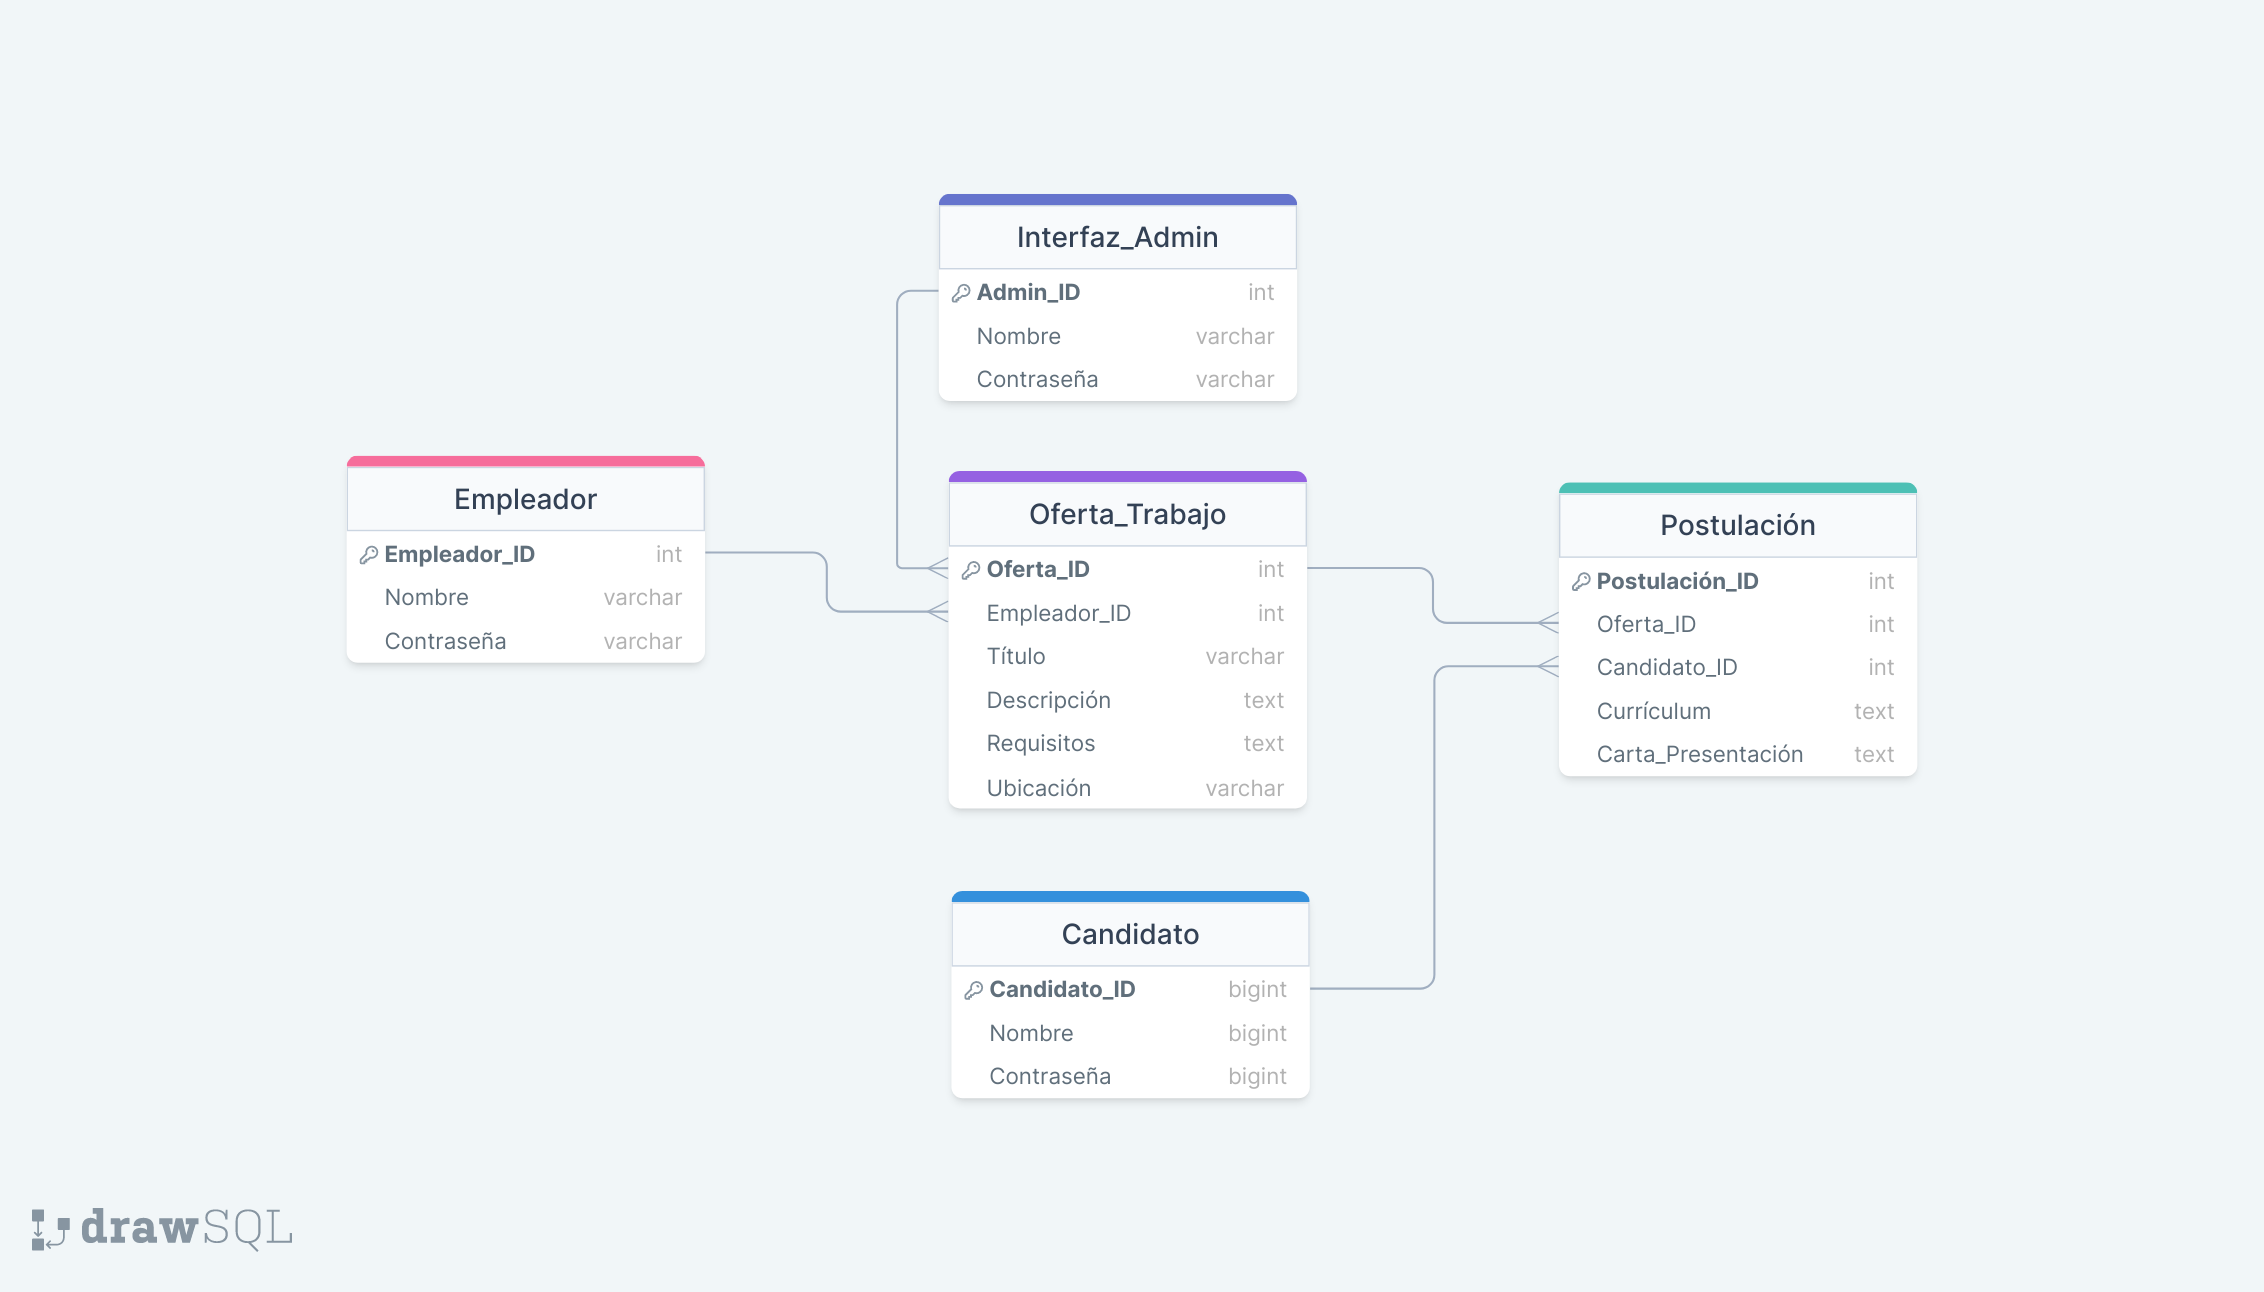
\includegraphics[width=0.9\textwidth]{img/diagrama.png}
        \caption{Diagrama entidad relación.}
        \label{fig:ejemplo}
    \end{figure}
    \newpage

    \subsection{Desarrollo del proyecto}
    \subsubsection{.gitignore}
    \begin{itemize}	
		\item Se creo el archivo \textbf{.gitignore} para no considerar los archivos \textbf{pycache, myvenv, db.sqlite3, etc.} que son innecesarios hacer seguimiento.
	\end{itemize}
	\begin{lstlisting}[language=bash,caption={Creando .gitignore}][H]
		$ vim lab05/.gitignore
	\end{lstlisting}
	\begin{lstlisting}[language=bash,caption={lab05/.gitignore}][H]
		*.pyc
      *~
      __pycache__
      myvenv
      db.sqlite3
      /static
      .DS_Store
	\end{lstlisting}
	\begin{lstlisting}[language=bash,caption={Commit de .gitignore}][H]
		$ git add .
		$ git commit -m "Creando .gitignore para lab05"			
		$ git push -u origin main
	\end{lstlisting}
    \subsubsection{jobs\_board/jobs\_board/accounts/admin.py}
    \begin{itemize}
        \item El código dado registra el modelo CustomUser en el panel de administracion de Django, lo que permite administrar y manipular los registros de usuario personalizados a través de una interfaz facil de usar.
    \end{itemize}
    \begin{lstlisting}[language=bash,caption={admin.py}][H]
		from django.contrib import admin

      # Register your models here.
      from .models import CustomUser

      admin.site.register(CustomUser)
	\end{lstlisting}
    \subsubsection{jobs\_board/jobs\_board/accounts/apps.py}
    \begin{itemize}
        \item Configura el tipo de campo automático predeterminado como 'django.db.models.BigAutoField' y establece el nombre de la aplicación como 'accounts'.
    \end{itemize}
    \begin{lstlisting}[language=bash,caption={apps.py}][H]
		from django.apps import AppConfig


      class AccountsConfig(AppConfig):
          default_auto_field = 'django.db.models.BigAutoField'
          name = 'accounts'
	\end{lstlisting}
 \subsubsection{jobs\_board/jobs\_board/accounts/forms.py}
    \begin{itemize}
        \item Los formularios necesarios para el inicio de sesión y el registro de usuarios en una aplicación Django.
    \end{itemize}
    \begin{lstlisting}[language=bash,caption={forms.py}][H]
     from django import forms
     from django.contrib.auth.forms import UserCreationForm
     from .models import CustomUser
     
     class LoginForm(forms.Form):
        email = forms.EmailField(label='Email')
        password = forms.CharField(label='Contraseña', widget=forms.PasswordInput)
        
     class RegistrationForm(UserCreationForm):
        email = forms.EmailField(label='Email')
        first_name = forms.CharField(label='Nombre')
        last_name = forms.CharField(label='Apellido')

     class Meta(UserCreationForm.Meta):
        model = CustomUser
        fields = ('email', 'first_name', 'last_name', 'password1', 'password2')
	\end{lstlisting}
    \subsubsection{jobs\_board/jobs\_board/accounts/migrations/0001\_initial.py}
    \begin{itemize}
        \item El modelo 'CustomUser' incluye campos como 'id', 'password', 'last\_login', 'is\_superuser', 'email', 'first\_name', 'last\_name', 'is\_active', 'is\_staff', 'date\_joined', 'groups' y 'user\_permissions'. Estos campos representan información relevante para la autenticación, autorización y gestión de usuarios en la aplicación.

        \item Además de la definición del modelo, el código establece opciones para el mismo, en este caso, se configura 'abstract' como 'False'.
    \end{itemize}
    \subsubsection{jobs\_board/jobs\_board/accounts/models.py}
    \begin{itemize}
        \item El modelo llamado CustomUser tiene campos como correo electrónico, nombre, apellido, estado de activación y fecha de registro. También incluye un administrador personalizado que proporciona métodos para crear usuarios normales y superusuarios.
        \item Además, el modelo establece que el correo electrónico se utilizará como campo de inicio de sesión en lugar del nombre de usuario. Tiene relaciones de muchos a muchos con grupos y permisos para asignarlos a los usuarios.
        
    \lstinputlisting[language=Python, caption={models.py},numbers=left,]{src/models.py}
    \end{itemize}
    \subsubsection{jobs\_board/jobs\_board/accounts/views.py}
    \begin{itemize}
        \item login\_view maneja el inicio de sesión de los usuarios. Verifica si el formulario de inicio de sesión es válido, autentica al usuario y lo redirige a la lista de trabajos si la autenticación es exitosa.

        \item register\_view se encarga del registro de nuevos usuarios. Guarda los datos del formulario de registro en la base de datos y redirige al usuario a la página de inicio de sesión.
        
    \lstinputlisting[language=Python, caption={views.py},numbers=left,]{src/views.py}
    \end{itemize}
    \subsubsection{jobs\_board/jobs\_board/jobs\_board/urls.py}
    \begin{itemize}
        \item La ruta 'admin/' apunta a las vistas proporcionadas por la aplicación de administración de Django.
        \item La ruta 'accounts/' incluye las URL definidas en el archivo urls.py de la aplicación accounts.
        \item La ruta '' (ruta vacía) muestra la vista definida en TemplateView con el nombre 'home.html', que representa la página de inicio de la aplicación.
        \item Además, se importa staticfiles\_urlpatterns para configurar correctamente los patrones de URL para servir archivos estáticos en modo de desarrollo.
        
    \lstinputlisting[language=Python, caption={urls.py},numbers=left,]{src/urls.py}
    \end{itemize}
    \subsubsection{templates/.html}
    \begin{itemize}
        \item  Incluimos un encabezado, el formulario con los campos de correo electrónico y contraseña, y un botón para enviar los datos del formulario.
    \lstinputlisting[language=HTML, caption={login.html},numbers=left,]{src/login.html}
    \item  Muy parecida a login, incluimos un encabezado, el formulario con los campos de correo electrónico y contraseña, y un botón para enviar los datos del formulario.
    \lstinputlisting[language=HTML, caption={register.html},numbers=left,]{src/register.html}
    \item  Estrcutura básica de Django.
    \lstinputlisting[language=HTML, caption={base.html},numbers=left,]{src/base.html}
    \item Se extiende de 'base.html' y muestra una página de inicio con dos botones: "Iniciar sesión" y "Registrarse". Los botones tienen enlaces dinámicos que se determinan utilizando las etiquetas .
    \lstinputlisting[language=HTML, caption={home.html},numbers=left,]{src/home.html}
    \end{itemize}
    \newpage
    \subsection{Avance del proyecto}
    \begin{itemize}
        \item Ahora veremos el aspecto visual de como se empieza a ver el proyecto:
        \begin{enumerate}
            \item \textbf{home.html} es lo primero que veran los usuarios al entrar a la página, en versiones futuras habrán más aspectos llamativos.
            \begin{figure}[h]
            \centering
            \fbox{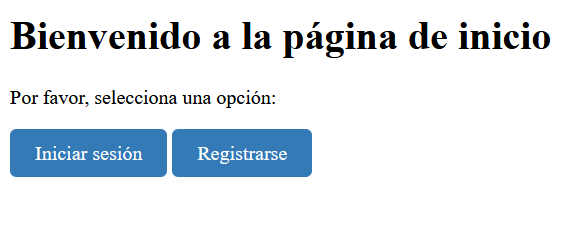
\includegraphics[width=0.7\textwidth]{img/home.png}}
            \caption{home}
            \label{fig:ejemplo}
            \end{figure}
            \item \textbf{login.html} es una de las opciones que tiene el usuario al ingresar a la pagina.
            \begin{figure}[h]
            \centering
            \fbox{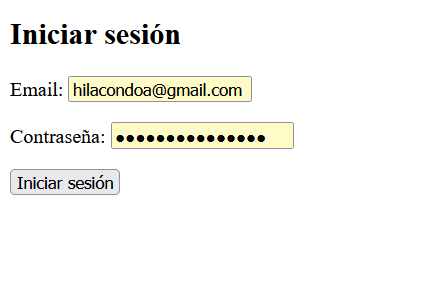
\includegraphics[width=0.7\textwidth]{img/login.png}}
            \caption{login}
            \label{fig:ejemplo}
            \end{figure}
\newpage
            \item \textbf{register.html} es otra de las opciones que tiene el usuario al ingresar a la pagina.
            \begin{figure}[h]
            \centering
            \fbox{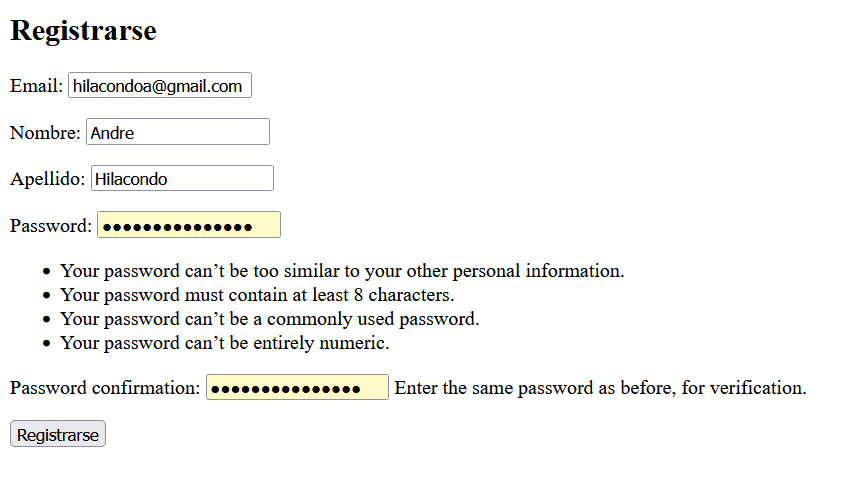
\includegraphics[width=0.9\textwidth]{img/register.png}}
            \caption{register}
            \label{fig:ejemplo}
            \end{figure}
        \end{enumerate}    
    \end{itemize}
    \subsection{Pregunta}
    \begin{itemize}
    \item Por cada integrante del equipo, resalte un aprendizaje que adquiri ́o al momento de estudiar Django. No se reprima de ser detallista. Coloque su nombre entre parentesis para saber que es su aporte.
    \begin{itemize}
        \item Implementé el sistema de registro de usuarios, tambien aprendí sobre el manejo de formularios en Django y cómo validar los datos de registro y ya por ultimo tambien aprendi sobre diseño de páginas y cómo crear una interfaz de registro atractiva \textbf{(Andre Hilacondo)}.
        \item Yo hice en la autenticación de usuarios, aprendí a utilizar el sistema de autenticación de Django y a diseñar la interfaz de inicio de sesión y aunque costo tambien aprendi cómo configurar las páginas de inicio de sesión y cierre de sesión correctamente \textbf{(GonzaloLayme)}.
        \item Sobre de la publicación de ofertas de trabajo, esa fue mi parte, aprendí a crear un formulario para que los empleadores puedan ingresar los detalles de las ofertas y también exploré cómo guardar los datos en la base de datos y cómo manejar la carga de imágenes relacionadas con las ofertas \textbf{(Andre Delgado)}.
        \item Me enfoque en la búsqueda de ofertas de trabajo para ello tuve que investigar otras platafromas parecidas y sacar lo mejor, descubrí cómo realizar consultas en la base de datos para filtrar y mostrar las ofertas de acuerdo a los criterios de búsqueda. Además, aprendí a clasificar las ofertas por categoría y a mejorar la eficiencia de las consultas \textbf{(Sebastian Chirinos)}.
        \item Me encargaron los detalles de las ofertas de trabajo, implementé la vista para mostrar la información detallada de cada oferta y a diseñar una interfaz atractiva para visualizar los detalles, también trabajé en la funcionalidad para mostrar de forma segura la información de contacto del empleador y CSS\textbf{(Gabriel Soto)}.
    \end{itemize}
    \end{itemize}   
    
	\subsection{Commits}
	\begin{lstlisting}[language=bash,caption={Commits del laboratorio}][H]
commit f621ef2f91afe924f3c828433764cd915f8d0a4b (HEAD -> ramaAndre, origin/ramaAndre)
Author: Andre Delgado <adelgadoal@unsa.edu.pe>
Date:   Mon Jun 19 22:01:40 2023 -0500

    super coommit
commit f621ef2f91afe924f3c828433764cd915f8d0a4b (HEAD -> ramaAndre, origin/ramaAndre)
Author: Andre Delgado <adelgadoal@unsa.edu.pe>
Date:   Mon Jun 19 22:01:40 2023 -0500

    super coommit

commit 66c783c5f6db75232ff466d7616f55731386aa99
Author: Andre Delgado <adelgadoal@unsa.edu.pe>
Date:   Mon Jun 19 22:00:15 2023 -0500

    commit3

commit 923e5c7d650e51cb4b0d5272a440fb36f902d5e6
Author: Andre Delgado <adelgadoal@unsa.edu.pe>
Date:   Mon Jun 19 21:57:05 2023 -0500

    commit

commit 57546aadec1ebcbc57e5ad50681a3b25a57ceb46 (origin/main, origin/HEAD, main)
Merge: c4126b2 af34c6d
Author: ahilacondo <ahilacondo@unsa.edu.pe>
Date:   Mon Jun 19 15:26:40 2023 -0500

    Cambios extras

commit af34c6d7e9f4d480d17d75847dc372b5ec475b92 (ramaHilacondo)
Author: ahilacondo <ahilacondo@unsa.edu.pe>
Date:   Mon Jun 19 15:23:07 2023 -0500

    Cambios extras

commit c4126b2d3b477897f9d1c8c8861acdbd20c36421
Author: ahilacondo <ahilacondo@unsa.edu.pe>
Date:   Mon Jun 19 15:20:43 2023 -0500

    Cambios extras

commit dd73bcc188c5b8db512110f98fb0dbab4552519a
Merge: 1c631e6 63d6000
:...skipping...
commit f621ef2f91afe924f3c828433764cd915f8d0a4b (HEAD -> ramaAndre, origin/ramaAndre)
Author: Andre Delgado <adelgadoal@unsa.edu.pe>
Date:   Mon Jun 19 22:01:40 2023 -0500

    super coommit

commit 66c783c5f6db75232ff466d7616f55731386aa99
Author: Andre Delgado <adelgadoal@unsa.edu.pe>
Date:   Mon Jun 19 22:00:15 2023 -0500

    commit3

commit 923e5c7d650e51cb4b0d5272a440fb36f902d5e6
Author: Andre Delgado <adelgadoal@unsa.edu.pe>
Date:   Mon Jun 19 21:57:05 2023 -0500

    commit

commit 57546aadec1ebcbc57e5ad50681a3b25a57ceb46 (origin/main, origin/HEAD, main)
Merge: c4126b2 af34c6d
Author: ahilacondo <ahilacondo@unsa.edu.pe>
Date:   Mon Jun 19 15:26:40 2023 -0500

    Cambios extras

commit af34c6d7e9f4d480d17d75847dc372b5ec475b92 (ramaHilacondo)
Author: ahilacondo <ahilacondo@unsa.edu.pe>
Date:   Mon Jun 19 15:23:07 2023 -0500

    Cambios extras

commit c4126b2d3b477897f9d1c8c8861acdbd20c36421
Author: ahilacondo <ahilacondo@unsa.edu.pe>
Date:   Mon Jun 19 15:20:43 2023 -0500

    Cambios extras

commit dd73bcc188c5b8db512110f98fb0dbab4552519a
Merge: 1c631e6 63d6000
Author: ahilacondo <ahilacondo@unsa.edu.pe>
Date:   Mon Jun 19 15:18:52 2023 -0500

    Merge branch 'ramaHilacondo'

commit 63d600027925968de44debafac0984f6cde5a53a (origin/ramaHilacondo)
Author: ahilacondo <ahilacondo@unsa.edu.pe>
Date:   Mon Jun 19 15:15:16 2023 -0500

    Diagrama entidad relación, y código de conducta

commit 1c631e6557c6ba99cd4cc83a10ba8c0ec5461992
Author: ahilacondo <ahilacondo@unsa.edu.pe>
Date:   Mon Jun 19 13:41:22 2023 -0500

    Cambios en el README.md

commit 41527080c7f0aed6b30395df1744d79962270ef0
Author: ahilacondo <ahilacondo@unsa.edu.pe>
Date:   Mon Jun 19 13:36:13 2023 -0500

    Iniciamos con el proyecto Job_board

commit f915221d0dd389e157814149276959e01e4bf957 (origin/andre-delgado)
Author: Gonzalo01703 <glaymem@unsa.edu.pe>
Date:   Sun Jun 18 22:35:54 2023 -0500

    .

commit f3cbcf6828cf03f6ed37b21a1e31255c4f6636c4
Author: Gonzalo01703 <glaymem@unsa.edu.pe>
Date:   Sun Jun 18 22:35:01 2023 -0500

    Se creo la plantilla base

commit 968ca7dcd53b518f101f3ca35213e0b292fb318f
Author: Gonzalo01703 <glaymem@unsa.edu.pe>
Date:   Sun Jun 18 22:31:31 2023 -0500

    Se estructura de como se trabajara

commit 35dc86f8f09be84f9c9fcf78049512daa5fbeb53
Author: GonzaloRail <132712920+GonzaloRail@users.noreply.github.com>
Date:   Fri Jun 16 14:53:11 2023 -0500

    Initial commit
    
	\end{lstlisting}
	
\subsection{Etapas finales del proyecto}
\begin{itemize}	
		\item Al proyecto le falta muchos detalles pero la estructura ya está definida al igual que las ideas a futuro, se investigara más sobre la interfaz atractiva y el uso de todo lo aprendido en programación web 2.
        \item Proyecto (actual):
         \begin{figure}[h]
        \centering
        
\includegraphics[width=0.9\textwidth]{img/home-2.jpeg}
        \caption{Proyecto "Jobs Board".}
        \label{fig:ejemplo}
    \end{figure}
	\end{itemize}
        
        
	\subsection{Estructura de laboratorio 04}
	\begin{itemize}	
		\item El contenido que se entrega en este laboratorio es el siguiente:
	\end{itemize}
\begin{lstlisting}[style=ascii-tree]
job_board/
├── job_board/
│   ├── __init__.py
│   ├── settings.py
│   ├── urls.py
│   └── wsgi.py
├── jobs/
│   ├── __init__.py
│   ├── admin.py
│   ├── models.py
│   ├── forms.py
│   ├── urls.py
│   └── views.py
├── templates/
│   └── jobs/
│       ├── job_list.html
│       └── job_detail.html
└── manage.py
\end{lstlisting}    

	

	\section{\textcolor{red}{Rúbricas}}
	
	\subsection{\textcolor{red}{Entregable Informe}}
	\begin{table}[H]
		\caption{Tipo de Informe}
		\setlength{\tabcolsep}{0.5em} % for the horizontal padding
		{\renewcommand{\arraystretch}{1.5}% for the vertical padding
		\begin{tabular}{|p{3cm}|p{12cm}|}
			\hline
			\multicolumn{2}{|c|}{\textbf{\textcolor{red}{Informe}}}  \\
			\hline 
			\textbf{\textcolor{red}{Latex}} & \textcolor{blue}{El informe está en formato PDF desde Latex,  con un formato limpio (buena presentación) y facil de leer.}   \\ 
			\hline 
			
			
		\end{tabular}
	}
	\end{table}
	
	\clearpage
	
	\subsection{\textcolor{red}{Rúbrica para el contenido del Informe y demostración}}
	\begin{itemize}			
		\item El alumno debe marcar o dejar en blanco en celdas de la columna \textbf{Checklist} si cumplio con el ítem correspondiente.
		\item Si un alumno supera la fecha de entrega,  su calificación será sobre la nota mínima aprobada, siempre y cuando cumpla con todos lo items.
		\item El alumno debe autocalificarse en la columna \textbf{Estudiante} de acuerdo a la siguiente tabla:
	
		\begin{table}[ht]
			\caption{Niveles de desempeño}
			\begin{center}
			\begin{tabular}{ccccc}
    			\hline
    			 & \multicolumn{4}{c}{Nivel}\\
    			\cline{1-5}
    			\textbf{Puntos} & Insatisfactorio 25\%& En Proceso 50\% & Satisfactorio 75\% & Sobresaliente 100\%\\
    			\textbf{2.0}&0.5&1.0&1.5&2.0\\
    			\textbf{4.0}&1.0&2.0&3.0&4.0\\
    		\hline
			\end{tabular}
		\end{center}
	\end{table}	
	
	\end{itemize}
	
	\begin{table}[H]
		\caption{Rúbrica para contenido del Informe y demostración}
		\setlength{\tabcolsep}{0.5em} % for the horizontal padding
		{\renewcommand{\arraystretch}{1.5}% for the vertical padding
		%\begin{center}
		\begin{tabular}{|p{2.7cm}|p{7cm}|x{1.3cm}|p{1.2cm}|p{1.5cm}|p{1.1cm}|}
			\hline
    		\multicolumn{2}{|c|}{Contenido y demostración} & Puntos & Checklist & Estudiante & Profesor\\
			\hline
			\textbf{1. GitHub} & Hay enlace URL activo del directorio para el  laboratorio hacia su repositorio GitHub con código fuente terminado y fácil de revisar. &2 &X &2 & \\ 
			\hline
			\textbf{2. Commits} &  Hay capturas de pantalla de los commits más importantes con sus explicaciones detalladas. (El profesor puede preguntar para refrendar calificación). &4 &X &4 & \\ 
			\hline 
			\textbf{3. Código fuente} &  Hay porciones de código fuente importantes con numeración y explicaciones detalladas de sus funciones. &2 &X &2 & \\ 
			\hline 
			\textbf{4. Ejecución} & Se incluyen ejecuciones/pruebas del código fuente  explicadas gradualmente. &2 &X &2 & \\ 
			\hline			
			\textbf{5. Pregunta} & Se responde con completitud a la pregunta formulada en la tarea.  (El profesor puede preguntar para refrendar calificación).  &2 &X &2 & \\ 
			\hline	
			\textbf{6. Fechas} & Las fechas de modificación del código fuente estan dentro de los plazos de fecha de entrega establecidos. &2 &X &2 & \\ 
			\hline 
			\textbf{7. Ortografía} & El documento no muestra errores ortográficos. &2 &X &2 & \\ 
			\hline 
			\textbf{8. Madurez} & El Informe muestra de manera general una evolución de la madurez del código fuente,  explicaciones puntuales pero precisas y un acabado impecable.   (El profesor puede preguntar para refrendar calificación).  &4 &X &4 & \\ 
			\hline
			\multicolumn{2}{|c|}{\textbf{Total}} &20 & &20 & \\ 
			\hline
		\end{tabular}
		%\end{center}
		%\label{tab:multicol}
		}
	\end{table}
	
\clearpage

\section{Referencias}
\begin{itemize}			
	\item \url{https://developer.mozilla.org/en-US/docs/Learn/Server-side/Django/Tutorial\_local\_
library\_website}
	\item \url{https://github.com/mdn/django-locallibrary-tutorial}
        \item \url{https://github.com/rescobedoq/pw2/tree/main/labs/lab05}
        \item \url{https://realpython.com/}
        \item William S. Vincent. (2022). Django for Beginners: Build websites with Python. Django 4.0.
leanpub.com. \href{http://library.lol/main/22AF742D96697DE55EF5F88B08F1AA86}{URL}
\end{itemize}	
	
%\clearpage
%\bibliographystyle{apalike}
%\bibliographystyle{IEEEtranN}
%\bibliography{bibliography}
			
\end{document}